%Diese Zeile bitte -nicht- aendern.
\documentclass[course=erap] {aspdoc}

%eigene Imports
\usepackage{amsfonts}
\usepackage{pgfplots}
\usepackage{ulem}
\usepackage{amssymb}
\usepackage{mathtools}
\usepackage{graphicx}
\pgfplotsset{compat=1.16}


%%%%%%%%%%%%%%%%%%%%%%%%%%%%%%%%%
%% TODO: Ersetzen Sie in den folgenden Zeilen die entsprechenden -Texte-
%% mit den richtigen Werten.
\newcommand{\theGroup}{233} % Beispiel: 42
\newcommand{\theNumber}{A316} % Beispiel: A123
\author{Ludwig Gröber \and Julian Pins \and Daniel Safyan}
\date{Sommersemester 2023} % Beispiel: Wintersemester 2019/20
%%%%%%%%%%%%%%%%%%%%%%%%%%%%%%%%%

% Diese Zeile bitte -nicht- aendern.
\title{Gruppe \theGroup{} -- Abgabe zu Aufgabe \theNumber}

\begin{document}
    \maketitle


    \section{Einleitung}\label{sec:einleitung}

    In den Bereichen der speziellen Relativitätstheorie~\cite{relativity}, Kosmologie~\cite{universum1,universum2} und allgemein bei der Berechnung von Wellen~\cite{linear_waves} gibt es zahlreiche Anwendungen, in denen die Berechnung des \textit{Areasinus Hyperbolicus oder} $arsinh(x)$ von großer Bedeutung ist.
    Ebenso wird die Funktion verwendet, um Küsten vor zerstörerischen Wellen zu warnen als auch um die Ausdehnung des Universums zu berechnen.~\cite{universum1,universum2}
    In diesen Anwendungsgebieten ist es wichtig, die Funktion schnell und genau zu berechnen.
    Im Folgenden werden Methoden zur genauen und effizienten Berechnung dieser vielseitigen Funktion vorgestellt und analysiert.
    \begin{figure}[h]
        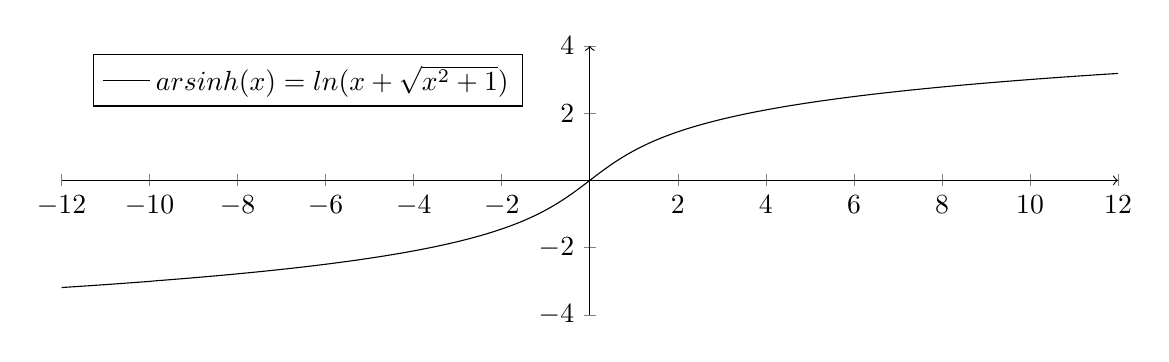
\begin{tikzpicture}[]
            \begin{axis}
                [
                legend pos = north west,
                width = 15 cm,
                height = 5 cm,
                xmin = -12, xmax = 12,
                ymin = -4, ymax = 4,
                axis lines=middle,
                axis line style={->},
                domain= -20: 20,
                samples = 500
                ]
                \addplot[] {ln(x + sqrt(x*x+1))};
                \legend{$arsinh(x) = ln(x + \sqrt{x^2 + 1})$}
            \end{axis}
        \end{tikzpicture}
        \caption{$arsinh(x)$-Funktionsplot}
    \end{figure}

    \subsection{Analyse und Spezifikation der Aufgabenstellung}\label{subsec:analyse-und-spezifikation-der-aufgabenstellung}

    Die Aufgabe A316 ist, den $arsinh(x)$ im C17 Standard von C zu approximieren.
    Spezifischer verlangt die Aufgabenstellung zwei Implementierungen, die auf einfachen arithmetischen Ausdrücken basieren sowie eine Vergleichsimplementierung, die komplexe Instruktionen benutzen darf.
    Eine der einfachen Implementierungen soll eine reine Reihe sein, während die andere einen Tabellen-Lookup benutzen soll.

    Für die Implementierungen wurden folgende Annahmen getroffen:
    Die \textbf{reine Reihenentwicklung} soll eine Berechnung der Form $\sum_{k=0}^{\pm\infty} a_k x^k$ sein und bis auf einzelne Inputs keine weiteren Fallunterscheidungen machen.
    Hierbei sollte eine Reihe gewählt werden, deren Konvergenzbereich am ehesten für ein mögliches Anwendungsgebiet geeignet ist.
    Als weitere Implementierung, die für alle Eingabewerte gültige Näherungen liefert, verwendet eine \textbf{Reihenentwicklung mit Fallunterscheidung} verschiedene Reihen in Abhängigkeit vom Eingabewert.
    Für die \textbf{Lookup-Tabelle} war der Speicherplatz Teil der zentralen Abwägung, da für die meisten Anwendungen Speichereffizienz wichtig ist.
    Zwischen den gespeicherten Werten soll linear interpoliert werden.
    Als \textbf{Vergleichsimplementierung} werden Funktionen der C math Bibliothek verwendet.
    Diese wird insbesondere für die Bewertung der Genauigkeit herangezogen.

    Diese vier Implementierungen werden in der Folge erklärt, auf Performanz und Genauigkeit untersucht, verglichen und anhand der Ergebnisse bewertet.


    \section{Lösungsansatz}\label{sec:losungsansatz}

    \subsection{Reihendarstellungen}\label{subsec:reihendarstellung}

    Bei der Approximation durch eine reine Reihe der Form $\sum_{k=0}^{\pm\infty} a_k x^k$ werden Overflows zum Problem.
    Unabhängig welche Reihe genutzt wird, können die Zwischenergebnisse $x^{\pm k}$ entweder für sehr große Werte oder sehr kleine Werte von $x$ nicht als $double$ dargestellt werden, was zu einem falschen Endergebnis führt.
    Daher haben solche Reihendarstellungen stets begrenzte Gültigkeitsbereiche.
    Es wird versucht, eine Reihenentwicklung zu finden, die für einen sinnvollen Konvergenzbereich möglichst genaue Ergebnisse liefert.

    Unter anderem kann die Methode der kleinsten Quadrate verwendet werden, um geeignet Koeffizienten für Reihenglieder mit positiven oder negativen Potenzen zu finden.
    Die auf diese Weise hergeleitete Reihenentwicklung liefert allerdings für Werte zwischen den verwendeten Datenpunkten zu ungenaue Ergebnisse.

    Daher wurden Reihenentwicklungen für verschiedene Intervalle hergeleitet, die im Folgenden näher erläutert werden sollen.
    Für bessere Verständlichkeit werden die drei Reihen mit \textit{TaylorArsinh}, \textit{TaylorLn} und \textit{Restreihe} bezeichnet.
    Die Berechnungen werden im Folgenden näher erläutert:

    \subsubsection{Reihendarstellung für $|x|\leq 1$}
    Für $|x| \leq 1$ wird die Taylor-Reihe des $arsinh(x)$ um den Entwicklungspunkt 0 \cite{taylor_series} verwendet:

    \[
        \textit{\textbf{TaylorArsinh}}\coloneqq arsinh(x) = \sum_{k = 0}^{\infty} \frac{(2k-1)!!(-x^2)^k}{(2k)!!(2k + 1)}
        = \sum_{k = 0}^{\infty} \frac{(-1)^k(2k)!x^{2k + 1}}{(2k + 1)(2^k*k!)^2}
    \]

    Das Auflösen der Doppelfakultäten liefert eine leichter implementierbare Formel.

    \subsubsection{Reihendarstellung für $|x|\geq 1$}
    Die Berechnung für $|x| > 1$ folgt aus folgender Näherung:
    \[
        arsinh(x) = \ln(x + \sqrt{x^2 + 1}) = \ln(2x) + error(x)
    \]

    Für die Berechnung von $\ln(2x)$ wird die Taylor-Reihe des natürlichen Logarithmus um den Entwicklungspunkt 1\cite{taylor_series} verwendet.
    Es ist zu beachten, dass diese Reihe ausschließlich im Wertebereich $[0, 2]$ konvergiert.
    \[
        \textbf{\textit{TaylorLn}}\coloneqq\ln(x) = \sum_{k = 1}^{\infty} \frac{(-1)^{k + 1}}{k}(x - 1)^k
    \]
    Der Fehler dieser Näherung kann durch eine dritte Reihe\cite{rest_series} berechnet werden, die vor allem für den Funktionswert von Eingabewerten $|x| < 2^{8}$ notwendig ist:
    \[
        \textit{\textbf{Restreihe}}\coloneqq error(x) =  \sum_{k = 1}^{\infty} \frac{(-1)^{k - 1}(2k)!}{2k(2^k\cdot k!)^2} \cdot \frac{1}{x^{2k}}
    \]

    \subsubsection{Optimierungen: Genauigkeit und Performanz}

    Die Koeffizienten einzelner Reihenglieder zu berechnen ist laufzeitintensiv, da insbesondere die Berechnung der Fakultät viel Zeit kostet.
    Daher lässt sich die Berechnung optimieren, indem die Koeffizienten aller drei Reihen bereits vor Runtime berechnet werden.
    Durch Anwendung des Horner-Schemas lassen sich die Reihen besonders effizient berechnen.

    Die Anzahl zu berechnender Reihengliedern, entsteht aus einer Abwägung zwischen Performanz und Genauigkeit.
    Wie viele Reihenglieder für ein möglichst genaues Ergebnis berechnet werden müssen, hängt von dem Eingabewert ab.
    Da die Reihenglieder aller drei Reihen für Eingabewerte innerhalb des jeweiligen Konvergenzbereichs immer kleiner werden, gilt:
    Je kleiner das letzte berechnete Reihenglied, desto genauer ist das Ergebnis.

    Wir betrachten zunächst \textit{TaylorArsinh}:
    Das k-te Reihenglied hat den Betrag
    \[
        \frac{(2k)!}{(2k + 1)(2^k*k!)^2}\cdot x^{2k+1}
    \]
    Aus dieser Formel lässt sich bereits ablesen, dass der Betrag des k-ten Reihengliedes kleiner ist, je kleiner $|x|$ ist.
    Die Reihe liefert demnach bereits mit weniger Reihengliedern genaue Ergebnisse, je näher x an 0 liegt.
    Mithilfe dieser Formel lässt sich feststellen, dass für $|x| = 0.25$ alle Reihenglieder ab dem 13. Glied keinen Einfluss mehr auf das Endergebnis haben, da sie aufgrund der Beschränkung der Mantisse auf 52 Bit diese bei der Addition absorbiert werden.
    Für $|x| = 0.5$ müssten 26 Reihenglieder berechnet werden.
    Für $|x| = 0.99$ sind bereits rund 1500 Reihenglieder nötig.
    Die Anzahl der zu berechnenden Reihenglieder wird auf 13 festgelegt und damit ein exponentiell ansteigender relativer Fehler ab $|x| > 0.25$ in Kauf genommen.
    Ähnliche Abwägungen lassen sich für die \textit{Restreihe} aufstellen, weshalb für diese Reihe ebenfalls 13 Reihenglieder verwendet werden.

    Es sei hier bereits erwähnt, dass ausgehend von diesen Untersuchungen eine weitere Optimierung umsetzbar wäre, die (beispielsweise mithilfe des Exponenten des Eingabewertes) die Anzahl der nötigen Reihenglieder bestimmt und nur diese berechnet.
    Durch diese Optimierung wird Overhead durch die Berechnung von für das Ergebnis irrelevanten Reihengliedern vermieden, auf Kosten eines geringen, festen Laufzeitanteils.

    \subsection{Reine Reihendarstellung}\label{subsec:reine-reihendarstellung}

    Es stellt sich die Frage, ob die Reihenentwicklung für $|x|\geq1$ oder $|x|\leq1$ verwendet werden sollte. Hierzu muss zwischen Genauigkeit und Nützlichkeit des Konvergenzbereichs abgewägt werden.

    Da im Datentyp double für $|x|<1$ gleich viele Werte existieren wie für $|x|\geq1$, beinhaltet der Konvergenzbereich der Reihen für die beiden Intervalle gleich viele mögliche double-Eingabewerte.

    Da es sich bei der Reihenentwicklung für $|x|\geq1$ nicht um eine reine Reihe handelt, gilt es zunächst, die beiden verwendeten Reihen zu einer reinen Reihe zu vereinigen:
    \[
        arsinh(x)\approx ln(2x) + error(x) = ln(2) - ln(\frac{1}{x}) + error(x)
    \]
    Da $|x|>1$ gilt, steht im Argument des natürlichen Logarithmus ein Wert $\in ]0, 1]$, für den die \textbf{TaylorLn}-Reihe konvergiert.
    Um die reine Reihe zu erhalten, können durch Ausmultiplizieren der ersten n Reihenglieder die ersten n Koeffizienten $a_k$ der neuen Reihe bestimmt werden, wodurch sich eine reine Reihendarstellung der Form $\sum_{k=0}^{n} a_k x^{-k}$ ergibt.

    Durch an dieser Stelle nicht weiter definerte Genauigkeits-Messungen hat sich ergeben, dass das Ergebnis dieser Näherung $ arsinh(x)\approx ln(2) - ln(\frac{1}{x}) + error(x)$ ungenauer wird, je größer $|x|$ ist.

    Da TaylorArsinh(x) hingegen für den Großteil der Eingabewerte unter 1 mit wenigen Reihengliedern bereits ein exaktes Ergebnis liefern kann,

    wird diese als Hauptimplementierung verwendet.


    \subsection{Reihendarstellung mit Fallunterscheidung}\label{subsec:reihendarstellung-mit-fallunterscheidung}

    Für die gemischte Reihenentwicklung wird zudem eine Fallunterscheidung nach den Eingabewerten getroffen, um für alle Eingabewerte eine möglichst genaue Näherung zu finden:
    \[ \operatorname{arsinh}(x) =
    \begin{cases}
        \textit{TaylorArsinh}     & \text{ falls } |x| < 1 \\
        \ln(2x) + error(x)  & \text{ falls } |x| >1 \\
        x     & \text{ falls } x \in \{\pm\inf, \pm Nan\}\\
    \end{cases}\]

    Für $|x|\geq1$ kann das $double$ Datenformat genutzt werden, um die Genauigkeit der Berechnung zu optimieren.
    Die Implementierung verwendet Exponent und Mantisse von $x$ um folgende Umformung zu treffen:
    \begin{gather*}
        x = M\cdot2^E \,\,\, mit \,\,\, M = implizierte Mantisse \,\,\, E = implizierter Exponent\\
        \ln(2x) = \ln(2) + \ln(x) = \ln(2) + \ln(M\cdot2^E) = \ln(2) + E\cdot\ln(2) + \ln(M)\\
    \end{gather*}
    Da $M\in[1, 2[$ liegt, kann \textit{TaylorLn} für die Berechnung von $\ln(M)$ verwendet werden.
    Für die so gegebenen Eingabewerte der Taylorreihe werden analog zu den Überlegungen in Kapitel 2.1.3 28 Reihenglieder für ein exaktes Ergebnis benötigt.

    \subsection{Tabellen-Lookup}
    Die Lookup-Tabelle speichert einige vorberechnete Werte der $arsinh$-Funktion und interpoliert für die verbleibenden Werte linear zwischen den beiden nächstgelegenen Tabellenwerten.
    Bei der Implementierung galt es zunächst, zwischen Speicherplatz der Tabelle und Genauigkeit des Ergebnisses abzuwägen.
    Im Rahmen der Ausarbeitung wurde ein Limit von 500KB für die Lookup-Tabelle festgelegt.
    Diese Größe ermöglicht das Speichern von rund 33000 Werten.
    Ebenso wurde eine logarithmische Verteilung der Werte festgelegt, da die Verteilung aller möglichen Werte im Datentyp $double$ logarithmisch ist.
    Für alle positiven Eingabewerte wurde für jeden möglichen Exponenten $[-1023, +1023]$ eine feste Anzahl an Werten vorberechnet.
    Das gesetzte Speicherlimit beschränkt die Genauigkeit auf 16 Werte pro Exponent.
    Folglich werden 32753 Werte gespeichert.
    Die Folgen dieser Designentscheidung werden im Kapitel Genauigkeit noch näher betrachtet.

    Diese Verteilung ermöglicht ein besonders effizientes Mapping der Eingabewerte auf den zugehörigen Index in der Lookup-Tabelle durch eine Hashfunktion.
    Durch eine Bitmaske lassen sich Exponent und die ersten 4 Bits der Mantisse ermitteln.
    Diese 15 bit bilden den Index $i$ des nächstkleineren Wertes in der Lookup-Tabelle.
    Mit diesem und dem nächsten Tabellenwert gilt $table[i] \leq arsinh(x) < table[i+1]$.
    Daraufhin wird gemäß
    \[
        arsinh(x) \approx \frac{x-x_i}{x_{i+1} - x_i}\cdot (y_{i+1}-y_i) + y_i
    \]
    linear interpoliert.
    Für negative Werte wird die Punktsymmetrie der $arsinh$-Funktion: $arsinh(-x) = -arsinh(x)$ genutzt\cite{properties}.
    Die Funktionswerte für negative Eingabewerte können per Fallunterscheidung mit $-arsinh(-x)$ berechnet werden, wodurch weniger Werte gespeichert werden müssen.

    \subsection{Implementierung mit komplexen Instruktionen}
    Die Vergleichsimplementierung kann unter Verwendung der C-Mathematikbibliothek die Formel $\ln{x+\sqrt{x^2+1}}$ direkt umsetzen. Ab etwa $|x|>10^{16}$ muss allerdings die Näherung $arsinh(x)\approx \ln{2x}$ herangezogen werden um double Overflows bei der Quadrierung zu vermeiden.

    \section{Genauigkeit}\label{sec:genauigkeit}

    \begin{figure}[h]
        \centering
        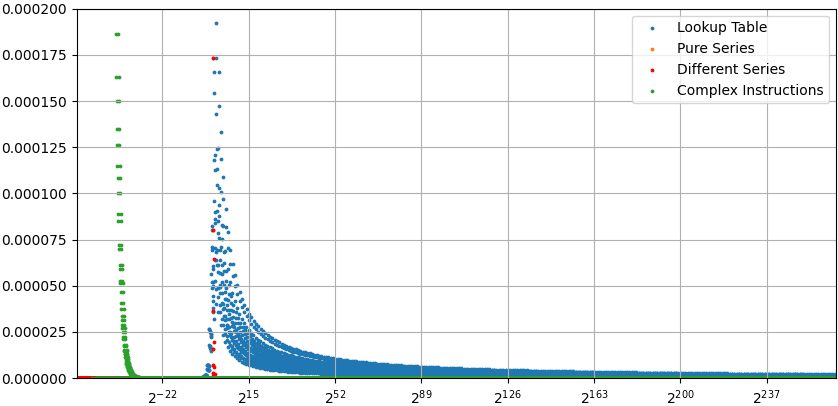
\includegraphics[width=12cm,height=5.5cm]{images/Figure3}
        \caption{rel. Fehler über positiven Wertebereich}
    \end{figure}


    Als Maßstab für die Genauigkeit der Ergebnisse wird im Folgenden der relative Fehler der Implementierung bezüglich des tatsächlichen mathematischen Funktionswerts verwendet.
    Die Diagramme wurden erstellt, indem für rund 40000 logarithmisch verteilte Eingabewerte der relative Fehler für alle vier Implementierungen errechnet und mittels $matplotlib$ aus $Python$ dargestellt wurde.

    \begin{figure}[htbp]
        \centering
        \begin{minipage}[b]{0.45\textwidth}
            \centering
            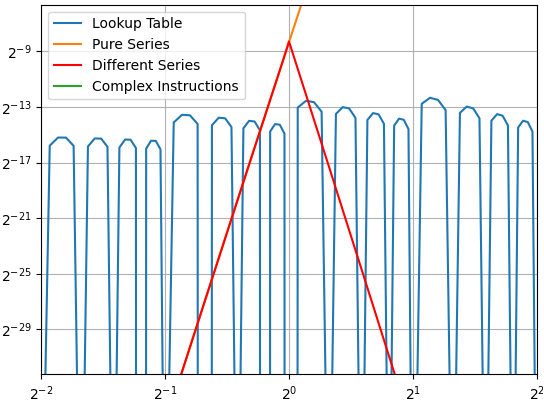
\includegraphics[width=\textwidth]{images/Figure1}
            \caption{rel. Fehler um 1}
        \end{minipage}
        \hfill
        \begin{minipage}[b]{0.45\textwidth}
            \centering
            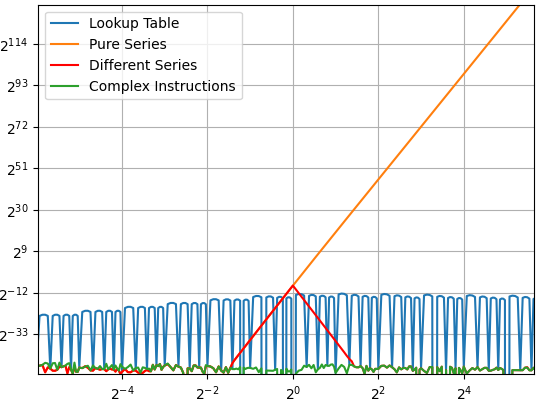
\includegraphics[width=\textwidth]{images/Figure2}
            \caption{rel. Fehler kleine x}
        \end{minipage}
    \end{figure}

    \subsection{Reine Reihenentwicklung}\label{subsec:reine-reihenentwicklung}
    
    Wie deutlich in Abb. 3 und 4 erkennbar ist, liefert die Reihenentwicklung für $|x|<0.25$ nahezu immer den exakten Funktionswert.
    Wie in Abb. 4 erkennbar, steigt der relative Fehler ab $|x| = 0.25$ exponentiell zum Eingabewert an.
    Dies lässt sich anhand der Konvergenz der Reihenglieder für verschiedene Eingabewerte erklären.
    Wie im Kapitel Optimierung erläutert, ist das Ergebnis genauer, je kleiner das letzte berechnete Reihenglied ist.
    Es wird gezeigt, dass bei 13 Reihengliedern die Grenze für die Entstehung von Ungenauigkeiten bei rund 0.25 liegt.
    Hierzu wird jeweils das letzte Reihenglied für x=0.25 berechnet:

    \[
        \textit{TaylorArsinh}: \frac{(2\cdot13)!0.25^{2\cdot13 + 1}}{(2\cdot13 + 1)(2^13\cdot13!)^2} \approx 2^{-59}
    \]

    Da das letzte Reihenglied noch unter $2^{-52}\cdot asinh(0.25)$ liegt und die Mantisse von doubles 52 bit beinhaltet, hat das Ergebnis noch maximale double Genauigkeit.
    Für größer werdende x-Werte, wird das letzte Reihenglied immer größer, wodurch der relative Fehler exponentiell ansteigt.
    Daher hat die reine Reihenentwicklung innerhalb ihres Konvergenzbereichs $|x|\leq1$ ihren maximalen relativen Fehler von circa $2^{-8} \approx 0.39\%$ am Eingabewert 1.
    Für das letzte (13.) berechnete Reihenglied für den Eingabewert 1 ergibt sich:

    \[
        \textit{TaylorArsinh}: \frac{(2\cdot13)!1^{2\cdot13 + 1}}{(2\cdot13 + 1)(2^13\cdot13!)^2} \approx 0.00574 \approx 2^{-8}
    \]

    Da das letzte Reihenglied die Größenordnung $2^{-8}$ hat, liegt der relative Fehler in dieser Größenordnung.
    Innerhalb ihres Konvergenzbereichs hat die reine Reihenentwicklung einen maximalen Fehler von $2^{-8}$.
    Außerhalb des Konvergenzbereichs $|x|\leq1$ konvergieren die einzelnen Reihenglieder nicht gegen 0, wodurch die Reihe nicht mehr anwendbar ist.
    Da das letzte Reihenglied weiter exponentiell ansteigt, steigt der relative Fehler exponentiell an, wie in Abb. 3 deutlich erkennbar.

    \subsection{Reihenentwicklung mit mehreren Reihen}\label{subsec:reihenentwicklung-mit-mehreren-reihen}

    In Abb. 2 und 4 lässt sich vergleichbar zur reinen Reihenentwicklung erkennen, dass die Reihenentwicklung außerhalb der Intervalle $0.25<|x|<4$ nahezu immer den exakten Funktionswert liefert.
    Es gibt einige Ausnahmen mit einem verschwindend geringen relativen Fehler $\leq2^{-50}$, welche sich durch floating-point-Rundungsfehler bei der Umrechnung der Polynomkoeffizienten erklären lassen.
    Da der Fall $1<x<0.25$ exakt äquivalent zu der reinen Reihe ist, wird die Ungenauigkeiten im Intervall $1<x<4$ betrachtet.
    Es wird das letzte Reihenglied der \textit{Restreihe} für $|x|=4$ berechnet.

    \[
        \textit{Restreihe}: \frac{(2\cdot13)!}{2\cdot13(2^{13}\cdot 13!)^2} \cdot \frac{1}{4^{2\cdot13}} \approx 2^{-59}
    \]

    Da das letzte Reihenglied unter $2^{-52}$ liegt, hat das Ergebnis noch maximale double Genauigkeit.
    Wie bei der reinen Reihe, wächst das letzte Reihenglied für x-Werte, die näher an 1 liegen exponentiell, was zu einem exponentiellen Anstieg des relativen Fehlers führt.
    Für das letzte Reihenglied für den Eingabewert 1 folgt:

    \[
        \textit{Restreihe}: \frac{(2\cdot13)!}{2\cdot13(2^{13}\cdot 13!)^2} \cdot \frac{1}{1^{2\cdot13}} \approx 0.00596 \approx 2^{-8}
    \]

    Da das letzte Reihenglied die Größenordnung $2^{-8}$ hat, stimmt der relative Fehler hier mit der reinen Reihe von der anderen Seite aus überein.

    \subsection{Lookup-Tabelle}\label{subsec:lookup-tabelle}

    Die Genauigkeit des Ergebnisses bei der Verwendung der Lookup-Tabelle hängt stark von den Eingabewerten ab.
    Ist der Eingabewert exakt einer der vorgespeicherten Werte in der Tabelle, so liefert die Funktion das exakte Ergebnis.
    Am ungenauesten ist die Funktion für Eingabewerte, die zwischen zwei gespeicherten Tabellenwerten liegen.
    Das lässt sich deutlich an der großen vertikalen Streuung der Fehlerwerte erkennen.

    Im Abb. 3 ist zudem deutlich erkennbar, dass die Funktion, wie die Reihenentwicklung, deutlich ungenauere Ergebnisse für Eingabewerte nahe an 1 liefert.
    Dies lässt sich mithilfe des Krümmungsverhaltens der Funktion begründen.
    Der folgende Graph zeigt die zweite Ableitung des $arsinh''(x) = \frac{-x}{x^2\cdot \sqrt{x^2+1}+\sqrt{x^2+1}}$:
    
    \begin{figure}
        \begin{tikzpicture}
            \begin{axis}
                [
                width = 15 cm,
                height = 5 cm,
                xmin = -10, xmax = 10,
                ymin = -0.5, ymax = 0.5,
                axis lines=middle,
                axis line style={->},
                domain= -20: 20,
                samples = 500,
                ]
                \addplot[] {-x/((x*x)* sqrt((x*x)+1) + sqrt((x*x)+1))};
                \addplot [color=blue, mark = *] coordinates {
                    (-0.707106781093, 0.3849001794598)
                };
                \addplot [color=blue, mark = *] coordinates {
                    (0.707106781093, -0.3849001794598)
                };
            \end{axis}
        \end{tikzpicture}
        \caption{$arsinh''(x)$}
    \end{figure}


    Der $arsinh(x)$ hat die maximale Krümmung bei circa $\pm 0.707$.
    Dementsprechend wird eine lineare Interpolation im Bereich dieser Stellen eine maximale Ungenauigkeit aufweisen.

    \subsection{Implementierung mit komplexen Instruktionen}\label{subsec:implementierung-mit-komplexen-instruktionen}

    Wie in Abb. 2 zu sehen ist, liefert die Implementierung mit komplexen mathematischen Instruktionen der C-Math Bibliothek für den Großteil des Wertebereichs den genauest möglichen Funktionswert für den Datentyp double.
    Die einzige Ausnahme bilden sehr kleine x-Werte.
    Dies lässt sich mit der Absorption beziehungsweise Auslöschung von Bits begründen, welche bei der Addition von doubles unterschiedlicher Größenordnung unvermeidbar auftritt.

    %TODO: Absorption bei doubles kann in zwei Sätzen erklärt werden
    Betrachten wird den Term $\sqrt{x^2 + 1}$ der allgemeinen Gleichung für den $arsinh(x)$.
    Ab $|x|<2^{-26}$ gilt stets $x^2<2^{-52}$. $x^2$ wird damit bei der Addition mit 1 vollständig absorbiert und $\sqrt{x^2 + 1}$ evaluiert zu 1.
    Hierdurch entsteht ein für kleinere $x$ immer größerer relativer Fehler.
    Ab $|x|<2^{-52}$ wird zudem x bei Addition auf 1 immer absorbiert, wodurch $\ln{(x+\sqrt{x^2 + 1})}$ automatisch zu 0 evaluiert.
    Für $|x|<2^{-52}$ ist die Implementierung mit komplexen mathematischen Instruktionen nicht anwendbar, da das Ergebnis (mit Ausnahme von 0) immer einen relativen Fehler von $100\%$ haben wird.


    \section{Performanzanalyse}\label{sec:performanzanalyse}

    Die Performanz der Implementierungen wird anhand der Laufzeit gemessen.
    Diese wird im Folgenden mit der Bibliothek $time.h$ gemessen.

    \subsection{Methodik und Annahmen}\label{subsec:methodik-und-annahmen}

    Gemessen wurde auf einem System mit Intel i5-10210U Prozessor, 1.60 GHz, 8 GiB Arbeitsspeicher, Ubuntu 22.04.2 LTS, 64 Bit, 5.19.0-46-generic Linux-Kernel.
    Kompiliert wurde mit GCC 11.3.0 mit der Option -O3. Um eine optimale Vergleichbarkeit der Ergebnisse zu garantieren, wurden alle nicht für das Betriebssystem nötigen Prozesse beendet.

    Da die Reihenentwicklung mit Fallunterscheidung zwei sehr verschiedene Berechnungen für $|x|<1$ und $|x|\geq 1$ durchführt, wurden bei der Laufzeitmessung diese beiden Fälle unterschieden. Aufgrund der Fallunterscheidung in der Implementierung mit komplexen Instruktionen wurde zudem der Fall $|x|>10^{16}$ abgegrenzt.
    Ansonsten hängt die Laufzeit aller drei Implementierungen bedingt von der Größenordnung der Eingabewerte ab, daher wurde die Laufzeitmessung für die beiden Intervalle jeweils mit repräsentativen Werten verschiedener Größenordnungen durchgeführt.
    Die Methoden wurden mit 10 verschiedenen Werten jeweils 100.000.000-fach aufgerufen, um das arithmetische Mittel der Zeit für einen Funktionsaufruf zu ermitteln.

    Abb. 6 zeigt die durchschnittliche Laufzeit eines Funktionsaufrufs der drei Implementierungen mit Reihenentwicklung, Tabellen-Lookup und der Implementierung mithilfe komplexer Instruktionen der C-math-library in Nanosekunden:

    \begin{figure}
        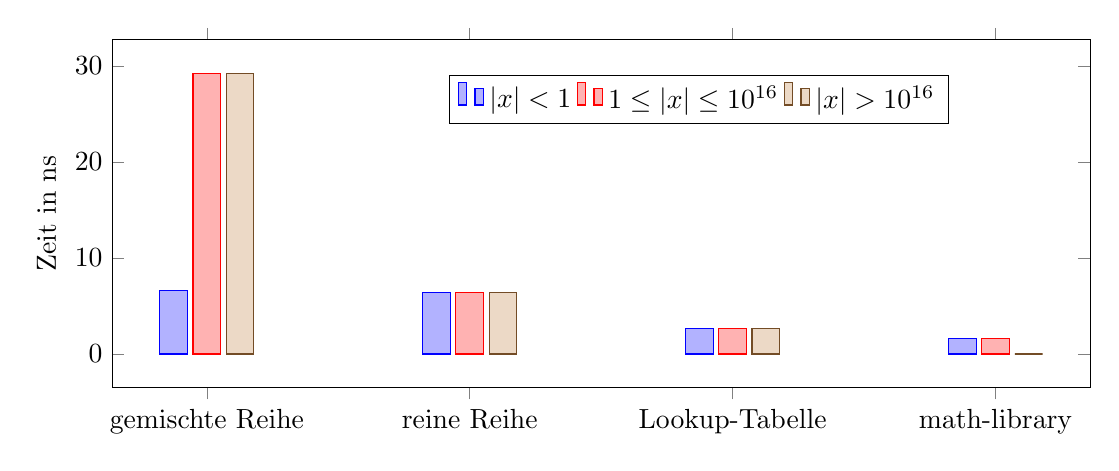
\begin{tikzpicture}
            \begin{axis}[
                width = 14 cm,
                height = 6 cm,
                ybar,
                enlargelimits = 0.12,
                symbolic x coords = {gemischte Reihe, reine Reihe,  Lookup-Tabelle,  math-library},
                xtick={gemischte Reihe, reine Reihe, Lookup-Tabelle, math-library},
                ylabel={Zeit in ns},
                legend style={at={(0.6, 0.9)},
                anchor=north,legend columns=-1},
            ]

                \addplot coordinates {(gemischte Reihe, 6.569) (reine Reihe,6.369) (Lookup-Tabelle, 2.613) (math-library, 1.648)};
                \addplot coordinates {(gemischte Reihe, 29.212) (reine Reihe, 6.369) (Lookup-Tabelle, 2.613) (math-library, 1.648)};
                \addplot coordinates {(gemischte Reihe, 29.212) (reine Reihe,6.369) (Lookup-Tabelle, 2.613) (math-library, 0.0)};
                \legend{$|x|<1$, $1\leq |x| \leq 10^{16}$, $|x|>10^{16}$};
            \end{axis}
        \end{tikzpicture}
        \caption{Laufzeit der Implementierungen}
    \end{figure}

    \subsection{Bewertung, Einordnung und Erklärung der Ergebnisse}\label{subsec:bewertung-einordnung-und-erklarung-der-ergebnisse}

    Wie in Abb. 6 zu sehen ist, gibt es starke Performanz-Unterschiede zwischen den verschiedenen Implementierungen.
    Es wird zunächst die Implementierung mit komplexen Instruktionen betrachtet.
    Diese ist hierbei im Vergleich zu den anderen Implementierungen deutlich schneller.
    Es offenbart sich innerhalb der Funktion eine signifikante Diskrepanz zwischen den Eingabewerten unterhalb von $10^{16}$ und jenen oberhalb von $10^{16}$.
    Ab dem gewählten Grenzwert von $10^{16}$ wird die Näherung $arsinh(x) = ln(2x)$ für die Berechnung verwendet.
    Diese Berechnung wird bei Optimierungsstufe $-O3$ so stark optimiert, dass sie sogar bei $10^{12}$ Iterationen eine Laufzeit nahe Null aufweist.
    Für den Großteil der Werte deren Betrag kleiner ist als $10^{16}$ sind allerdings neben der Logarithmus berechnung zudem Multiplikation, Addition und Wurzelberechnung für die exakte Berechnung erforderlich, wodurch die Funktion in diesem Intervall eine durchschnittliche Laufzeit von rund 1.648 ns hat.

    Die Lookup-Tabelle hat für alle reellen Eingabewerte eine ähnliche Laufzeit von 2.613 ns, da die Berechnung unabhängig von der Höhe des Eingabewerts ist.
    Durch die effiziente Hashfunktion mittels Bitmaske, die für das Mapping der Eingabewerte auf den jeweiligen Tabellenwert verwendet wird, ist diese Implementierung lediglich um den Faktor 1,5 langsamer, als die worst-case Laufzeit der Implementierung mit komplexen Instruktionen.
    Neben der Hashfunktion werden wenige einfache Instruktionen für die lineare Interpolation benötigt, was ebenfalls zu der hohen Performanz dieser Implementierung beiträgt.

    Im Vergleich zu der Lookup-Tabelle, braucht die reine Reihenentwicklung für die definierte Anzahl berechneter Reihenglieder mit 6.369 ns 2.5-mal so lange wie die Lookup-Tabelle.
    Dies ist damit zu begründen, dass die Reihenentwicklung deutlich mehr Multiplikationen und Summen über mehrere Reihenglieder verwendet, wodurch die Berechnung länger dauert.

    Die Reihendarstellung mit verschiedenen Reihen benötigt für $|x|<1$ ähnlich gleich viel Zeit wie die reine Reihenentwicklung, da derselbe Algorithmus wiederverwendet wird.
    Für die Approximation der Eingabewerte $|x|\geq1$ werden allerdings zwei verschiedene Reihen (TaylorLn und Restreihe) sowie einige komplexere Bitoperationen verwendet.
    Hierdurch benötigt diese Implementierung für $|x|\geq1$ rund 29.212 ns und damit 12-mal so lange wie die Lookup-Tabelle.
    Um eine vergleichbare Genauigkeit mit den Eingabewerten $|x|<1$ zu erhalten, sind diese Operationen allerdings notwendig.


    \section{Zusammenfassung und Ausblick}\label{sec:zusammenfassung-und-ausblick}

    \subsection{Zusammenfassung}\label{subsec:zusammenfassung}

    Der Trade-off zwischen Performance, Genauigkeit und Speicherverbrauch ist für die Implementierungen mit einer Lookup-Tabelle beziehungsweise einer Reihenentwicklung sehr unterschiedlich.
    Die Lookup-Tabelle ist schnell, benötigt allerdings mehr Speicherplatz, um genauere Werte zu erzielen.
    Eine Implementierung mit rund 30000 gespeicherten Werten, hat einen maximalen relativen Fehler von 0.02\%.

    Die reine Reihenentwicklung auf der anderen Seite liefert mit 13 brechneten Reihengliedern für den Großteil der Eingabewerte im Intervall $[-1, 1]$ den exakten Funktionswert und wird für Eingabewerte nahe an Eins ungenau.
    Da die Berechnungen in der Regel nicht auf ein bestimmtes Eingabeintervall beschränkt sind, ist von der Verwendung einer reinen Reihendarstellung abzuraten.
    

    Die gemischte Reihe liefert für 99,8\% aller doubles den exakten Funktionswert.
    Die Reihenentwicklung verglichen mit dem Lookup benötigt für $|x|>1$ die bis zu 11-fache Zeit für die Berechnung, andererseits verbraucht diese über 600-mal weniger Speicherplatz für eine genauere Berechnung.


    \subsection{Ausblick}\label{subsec:ausblick}

    Die Implementierung des $arsinh(x)$ war auf eine reine Reihenentwicklung und eine einfache Lookup-Tabelle mit linearer Näherung beschränkt.
    Unter weniger strengen Rahmenbedingungen ließe sich die Implementierung allerdings sowohl in Bezug auf Laufzeit, als auch Genauigkeit noch signifikant optimieren.

    Insgesamt kann die Reihendarstellung für solche Werte verwendet werden, für die nur wenige Reihenglieder berechnet werden müssen, um Speicherplatz für Lookuptabellenwerte zu sparen. 
    Für die übrigen Werte ist die Lookuptabelle allerdings in Bezug auf Laufzeit die bessere Wahl. 
    
    Für eine genauere Interpolation zwischen den gespeicherten Werten bietet sich die Verwendung von Splines in der Lookuptabelle an:
    Statt der bisher linearen Näherung zwischen zwei Messpunkten würde der $arsinh(x)$ in diesem Intervall durch ein Polynom angenähert.
    Hierzu werden in der Regel Polynome vom Grad drei verwendet.~\cite{splines}

    Des Weiteren ist eine effizientere Verteilung der Tabellenwerte möglich.
    Stärkere Krümmung der $arsinh$-Funktion führt zu ungenaueren Ergebnissen der Interpolation.
    Durch eine höhere Dichte an Messpunkten an stark gekrümmten Stellen und eine geeignete Mappingfunktion, würde die Lookup-Tabelle bei der gleichen Anzahl an vorgespeicherten Werten deutlich genauere Ergebnisse liefern.

    Durch dieses Verfahren verbessert sich die Genauigkeit, während sich die Laufzeit minimal erhöht.
    Zwar müssen für jedes Intervall mehrere Koeffizienten gespeichert werden, durch die effizientere Verteilung kann allerdings die Anzahl der Intervalle reduziert werden. 
    \newline
    \newline
    Zusammenfassend lässt sich feststellen, dass die Wahl der geeigneten Implementierung von den genauen Rahmenbedingungen abhängt.
    Die $arsinh$-Funktion findet in erster Linie Anwendung in verschiedensten Bereichen der Physik und Ingenierswissenschaften.
    Für die Verwendung in Echtzeitsystemen eignet sich somit die Lookup-Tabelle besser, da Messungen in der Regel kleine Fehler aufweisen und die Lookup-Tabelle für viele Werte aufgrund der höheren Performanz schneller Ergebnisse liefert.
    Steht Genauigkeit im Vordergrund, so eignet sich eine Reihenentwicklung mit einer geeigneten Menge an Reihengliedern besser.

    % TODO: Fuegen Sie Ihre Quellen der Datei Ausarbeitung.bib hinzu
    % Referenzieren Sie diese dann mit \cite{}.
    % Beispiel: CR2 ist ein Register der x86-Architektur~\cite{intel2017man}.
    \bibliographystyle{plain}
    \bibliography{Ausarbeitung}
    % Sämtliche in der Ausarbeitung verwendeten Quellen sind hier aufzuführen.
    % Es sollen nur zitierfähige Quellen verwendet werden. Wir empfehlen die Verwendung von BibTEX.

\end{document}